\documentclass[12pt, TexShade, letterpaper]{report}

\usepackage{import}
\import{}{preamble.tex}

\begin{document}

\begin{titlepage}
		\begin{center}
			\vspace*{0.5cm}

			\LARGE
			\textbf{Design and Analysis of 2x2 Cross-Over Trials}
			
			\vspace{1cm}
			
			\textit{Jules Lanari-Collard}
			
			\vspace{1.2cm}
			
			
\includegraphics[width=0.25\textwidth]{mcglogo.png}
			
			\Large
			MATH 410 Final Report
			
			\vspace{-5mm}
			McGill University
			
			\vspace{-5mm}
			Montr\'eal, Qu\'ebec, Canada
			
			\vspace{5mm}
			August 9, 2024
			\small
			\vspace{0.5cm}
			{\color{red} \hrule height 0.75mm}
			
			\vspace{0.2cm}
			
			Supervised by Dr. José Correa
		\end{center}
\end{titlepage}

\setlength{\voffset}{2cm}
\renewcommand{\chaptermark}[1]{%
	\markboth{\thechapter.\ #1}{}}
\chapter*{Abstract}\markboth{Abstract}{}
	\label{chap:engAbstract}
%	\addcontentsline{toc}{section}{\nameref{chap:engAbstract}}

 % Start of ToC, LoT, gls
	\tableofcontents\thispagestyle{plain}

 	\clearpage
	\pagenumbering{arabic} % restart page numbers at one, now in arabic style

	% start of mainmatter
\chapter{Introduction to Cross-over Trials}
\section{The Cross-over Design}
A cross-over trial is defined as a "trial in which subjects are given sequences of treatments with the object of studying differences between individual treatments" \cite{senn2002crossover}. This differs from the traditional parallel group trial, where subjects typically only receive one treatment throughout the trial.

The most common and simple cross-over design, is the 2x2 cross-over design, whereby there exist two treatments and two treatment groups. In this design, for example comparing two treatments \textit{A} and \textit{B}, subjects receive either \textit{A} or \textit{B} in the first period, and then are 'crossed over' to the other treatment in the second period. When only investigating the effects of one treatment (as opposed to comparing two treatments), the other 'treatment' is then a placebo.

Cross-over designs are typically used for testing treatments for ongoing or chronic diseases, where "there is no question of curing the underlying problem which has caused the illness but a hope of moderating its effects through treatment" \cite{senn2002crossover}. Examples of such conditions include asthma, rheumatism, epilepsy and migraines. Due to time constraints and the risk of drop-out or carryover, cross-over designs are more suitable to single-dose trials, as opposed to trials involving multiple doses over a period of time \cite{senn2002crossover}.

\subsection{Consequences}
A unique characteristic of the cross-over design is that only the \textit{order} of treatment is randomised, which has the following consequences \cite{piantadosi2005clinical}:
\begin{itemize}
    \item The validity of treatment comparison does not depend on randomisation.
    \item Randomisation does not guarantee an unbiased comparison of treatments.
    \item Treatment groups differ with respect to their recent exposure to potentially effective treatments.
\end{itemize}
In conclusion, the primary issue is that the comparability of treatments is not guaranteed by the structure of the trial alone, but instead depends on the treatments themselves \cite{piantadosi2005clinical}.

\section{Advantages}
The principal advantage of a cross-over design is that it can lead to significant savings in resources \cite{senn2002crossover}. Firstly, when compared to a parallel group trial, a cross-over design only requires half as many subjects to obtain the same number of observations per treatment.

Secondly, the data can be interpreted in terms of subject-level \textit{difference to control}, eliminating between-patient variation \cite{senn2002crossover}, which is usually greater than within-patient variation \cite{piantadosi2005clinical}. This reduces the number of observations (and hence subjects) required for the same precision in estimation. Furthermore, within-subject responses to treatments are usually positively correlated \cite{piantadosi2005clinical}, reducing the variance of the estimated treatment difference (from control) and increasing efficiency, as demonstrated below:

\begin{quote}
    \textit{Noticing that:}
\end{quote}
\begin{equation*}
    cov(\bar{Y}_A, \bar{Y}_B)
= \rho_{AB}sd(\bar{Y}_A)sd(\bar{Y}_B) = \rho_{AB} \cdot \frac{\sigma}{\sqrt{n}} \cdot \frac{\sigma}{\sqrt{n}} = \rho_{AB}\frac{\sigma^2}{n}
\end{equation*}
\begin{quote}
    \textit{Assuming constant variance in observations between patients and no period or carryover effects, we then have:}
\end{quote}
\begin{align*}
    var(\hat{\delta}_{AB}) &=
    \frac{\sigma^2}{n} + \frac{\sigma^2}{n} - 2cov(\bar{Y}_A, \bar{Y}_B) \\
    &= 2\frac{\sigma^2}{n}(1-\rho_{AB})
\end{align*}
\begin{quote}
    \textit{Where $\sigma^2$ is the observation variance, $\bar{Y}_A$ and $\bar{Y}_B$ are the average observations for treatments A and B respectively, $\rho_{AB}$ is the within-subject response correlation, and $\hat{\delta}_{AB} := \bar{Y}_A - \bar{Y}_B$.}

    Given that $\rho_{AB} = 0$ in parallel group trials, positive correlation of within-subject responses will make a crossover trial more efficient \cite{piantadosi2005clinical}.
\end{quote}

An oft-overlooked benefit to the crossover trial is improved recruitment and reduced spill-over rates \cite{piantadosi2005clinical}. Since all subjects are guaranteed to receive each treatment at least once, it can be easier to recruit participants. Furthermore, if a treatment is known to be desirable (e.g. exercise), parallel group trials can be subject to spill-over, where subjects in the control group voluntarily take the treatment. Cross-over trials are evidently less at risk of this, since all subjects know they will receive the treatment.

\section{Disadvantages}
Many of the aforementioned benefits of the crossover design come with drawbacks. For example, the longer trial and multiple treatments could be seen as an added inconvenience to patients, and analysis of results is often more difficult and complex (particularly when there are more than two treatments or groups). Also, the design cannot be used for infectious diseases, where either a significant deterioration or improvement in condition can occur during treatment, introducing bias into the subsequent treatment period. Patient drop-out is also very harmful to cross-over trials, since observations for all treatments are required for each patient to analyse the within-patient differences. In comparison, a parallel group trial can still recover some information after a patient drops out \cite{senn2002crossover}.

There is also risk of \textit{period-by-treatment interaction} complicating analysis, where the effect of the treatment is not constant over time \cite{senn2002crossover}. In other words, when the period in which the treatment is administered affects the effectiveness of the treatment.

\subsection{Carryover}
The most common example of a period-by-treatment interaction is carryover, defined as "the persistence of a treatment applied in one period in a subsequent period of treatment" \cite{senn2002crossover}. In a cross-over design, this occurs when at the beginning of the second treatment period, patients are not in the state they would have been in, had they not received treatment in the first period. This causes the effect of one treatment to be misinterpreted as the effect of both treatments combined, introducing bias to the treatment effect estimates.

Carryover is both difficult to test for and then to adjust for. Tests for carryover effects are difficult to interpret independently of the treatment effect, and including carryover parameters in the model introduces additional uncertainty and requires additional (usually unreasonable) assumptions \cite{senn2002crossover}.

\subsection{Wash-out Period}
Senn [2002] proposes that the most efficient way to deal with carryover is introducing a \textit{wash-out period} to the experiment design. A wash-out period is "a period in a trial during which the effect of a treatment given previously is believed to disappear" \cite{senn2002crossover}. After the wash-out period, we can assume that all measurements taken are no longer affected by the previous treatment, the consequence being that all conclusions become conditional on the absence of a carryover effect.

\chapter{Summary \& Visualisation of Cross-over Data} \label{visualisation}
This chapter will follow example data from Jones and Kenward \cite{jones2003design}, on a study testing efficacy of a drug (A) and a placebo (B) on patients with \textit{chronic obstructive pulmonary disease} (COPD). Due to the nature of the condition, the observation measurement used was \textit{peak expiratory flow rate} (PEFR), defined as "a simple measure of the maximal flow rate that can be achieved during forceful expiration following full inspiration" \cite{peakflowrate2023}. The study employed a 2x2 cross-over design on 56 patients, where each patient measured their PEFR 3 times per day during the treatment periods, recording the highest value. A sub-sample of the data is outlined in table \ref{pefData}.

\begin{table}[h]
\centering
\caption{Mean PEFR (L/min)}
\centering
\begin{tabular}[t]{l|l|l|r|r}
\hline
\textbf{Sequence} & \textbf{Subject} &
\textbf{Subject Label} & \textbf{Period 1} & \textbf{Period 2}\\
\hline
AB & 1 & 7 & 121.905 & 116.667\\
\hline
AB & 2 & 8 & 218.500 & 200.500\\
\hline
AB & 3 & 9 & 235.000 & 217.143\\
\hline
AB & 4 & 13 & 250.000 & 196.429\\
\hline
AB & 5 & 14 & 186.190 & 185.500\\
\hline
AB & 6 & 15 & 231.563 & 221.842\\
\hline
AB & 7 & 17 & 443.250 & 420.500\\
\hline
AB & 8 & 21 & 198.421 & 207.692\\
\hline
AB & 9 & 22 & 270.500 & 213.158\\
\hline
AB & 10 & 28 & 360.476 & 384.000\\
\hline
\end{tabular}
\label{pefData}
\end{table}
\section{Summarising Results}
When the outcome data is continuous, a simple summary table showing the mean and standard deviation of the outcomes \cite{vetter2017descriptive}, grouped by sequence and period (see table \ref{summaryTable}), suffices to give an overview of the data.  If further data were collected on additional covariates, they can be summarised using the traditional \textit{Table 1}.
\begin{table}
\centering
\caption{PEFR Results Summary (L/min)}
\centering
\begin{tabular}[t]{l|r|r|r|r|r}
\hline
Sequence & Subjects & Mean PEFR Period 1 & SD PEFR Period 1 & Mean PEFR Period 2 & SD PEFR Period 2\\
\hline
AB & 27 & 245.8387 & 82.77956 & 239.2033 & 81.69683\\
\hline
BA & 29 & 215.9919 & 72.62905 & 230.1617 & 73.94153\\
\hline
\end{tabular}
\end{table}


\section{Summary Plots}
Before undertaking any analysis, it is important to gain an understanding of the data and preliminary results. This section demonstrates the introductory plots suggested by Jones and Kenward \cite{jones2003design} for cross-over trials.

An overview of the trial data can be obtained using a simple boxplot, separated by sequence, as shown in figure \ref{fig:boxplot}.

\begin{figure}[ht]
    \centering
    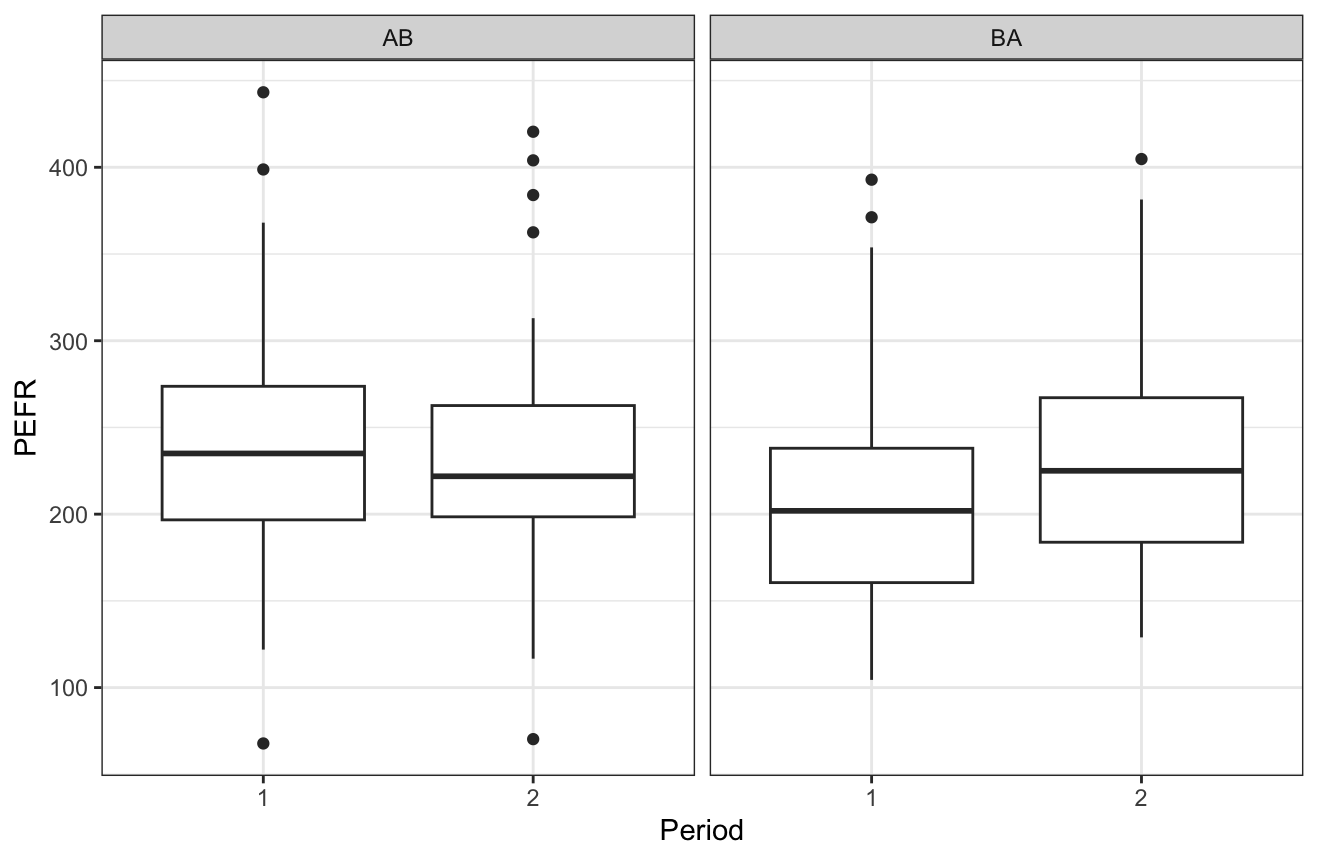
\includegraphics[width=0.85\linewidth]{report/figures/boxplot.png}
    \caption{Boxplot}
    \label{fig:boxplot}
\end{figure}

To begin to understand potential treatment effects, we can use a simple scatter plot of observations in each period, separated by group, as demonstrated in figure \ref{fig:period2vsperiod1}. Also included is a straight line with slope 1 and intercept 0; if the treatments were identical we would expect all observations to lie along this line. Using this plot we can verify within-patient correlation, and also notice the spread of points across the line, indicating between-patient variation.

\begin{figure}[ht]
    \centering
    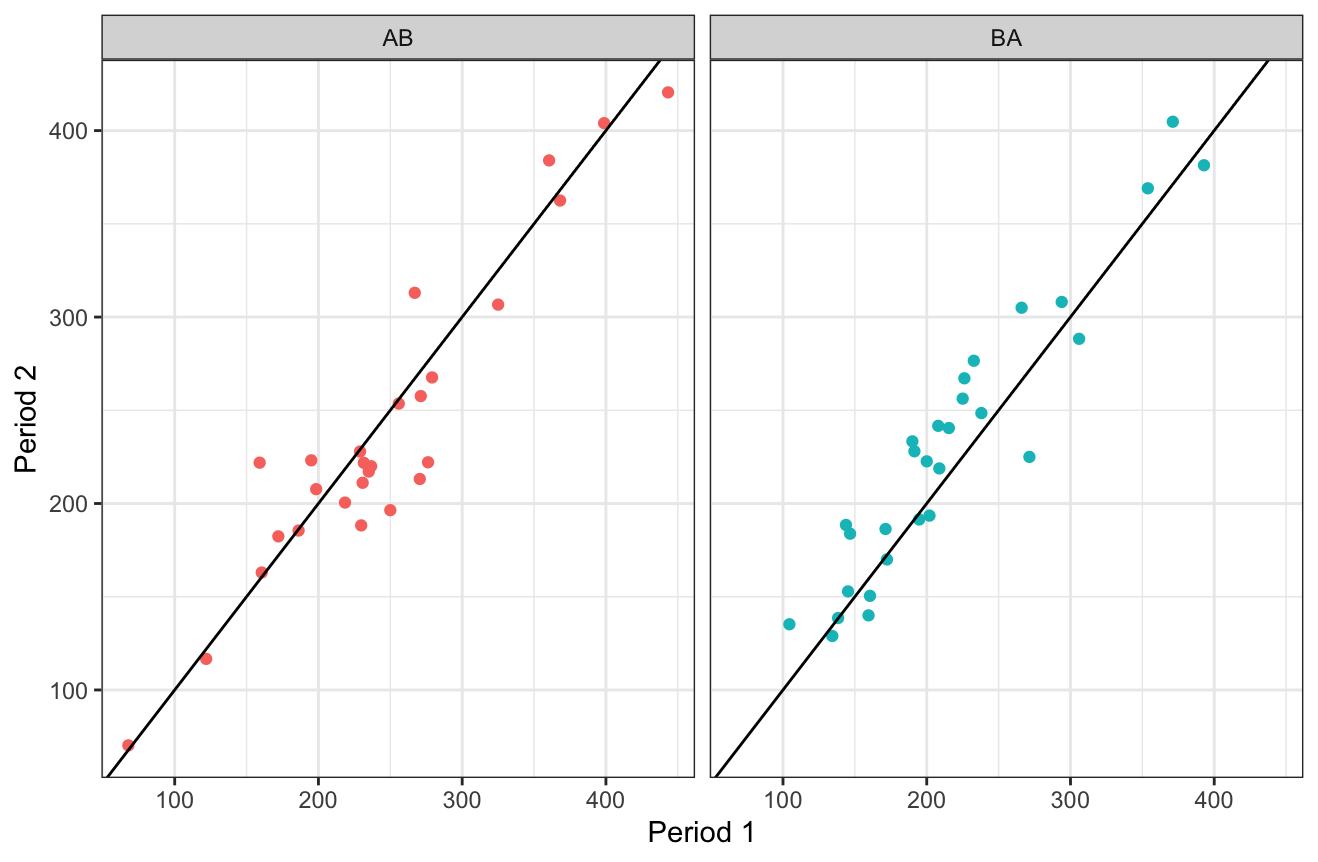
\includegraphics[width=0.85\linewidth]{report/figures/periodsPlot.png}
    \caption{Period 2 vs Period 1 Plots}
    \label{fig:period2vsperiod1}
\end{figure}

Additionally, we can overlay these two plots, distinguishing the groups using colour, and also including the centroids for each group, as demonstrated in figure \ref{fig:centroids}. This allows us to make some preliminary conclusions:
\begin{itemize}
    \item Both groups appearing symmetrical about the diagonal line suggests absence of a period effect.
    \item Centroids appearing on opposite sides of the line, with some vertical separation, suggests there exists a direct treatment effect.
\end{itemize}

\begin{figure}[ht]
    \centering
    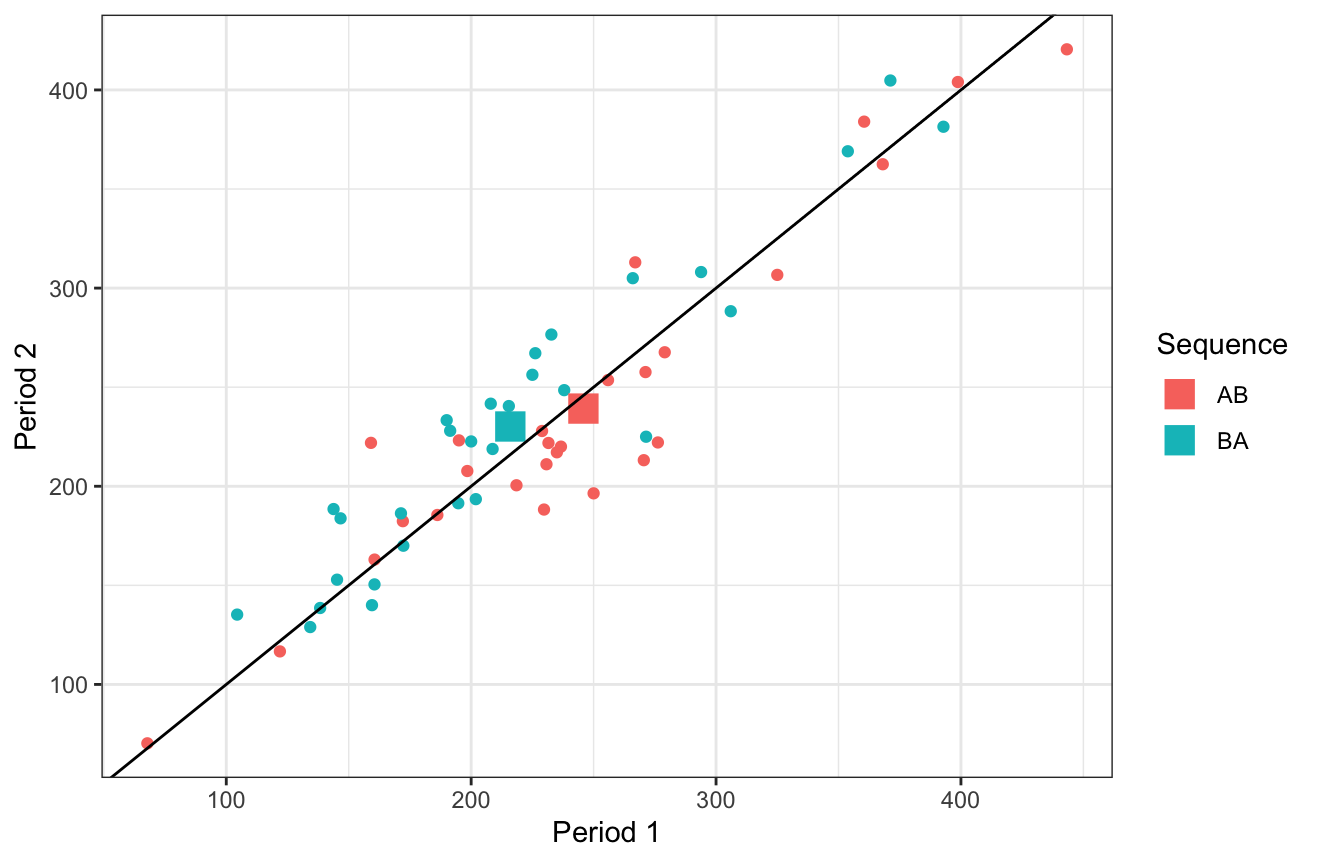
\includegraphics[width=0.85\linewidth]{report/figures/centroidsPlot.png}
    \caption{Period 2 vs Period 1 with Centroids}
    \label{fig:centroids}
\end{figure}

A plot which clearly shows the within-patient differences is the subject-profile plot, demonstrated in figure \ref{fig:subjectprofile}. This plot also allows us to visualise both within-patient and between-patient variability. It can also be combined with the boxplot to provide a comprehensive overview of the data, as shown in figure \ref{fig:pairedboxplot}.

\begin{figure}[ht]
    \centering
    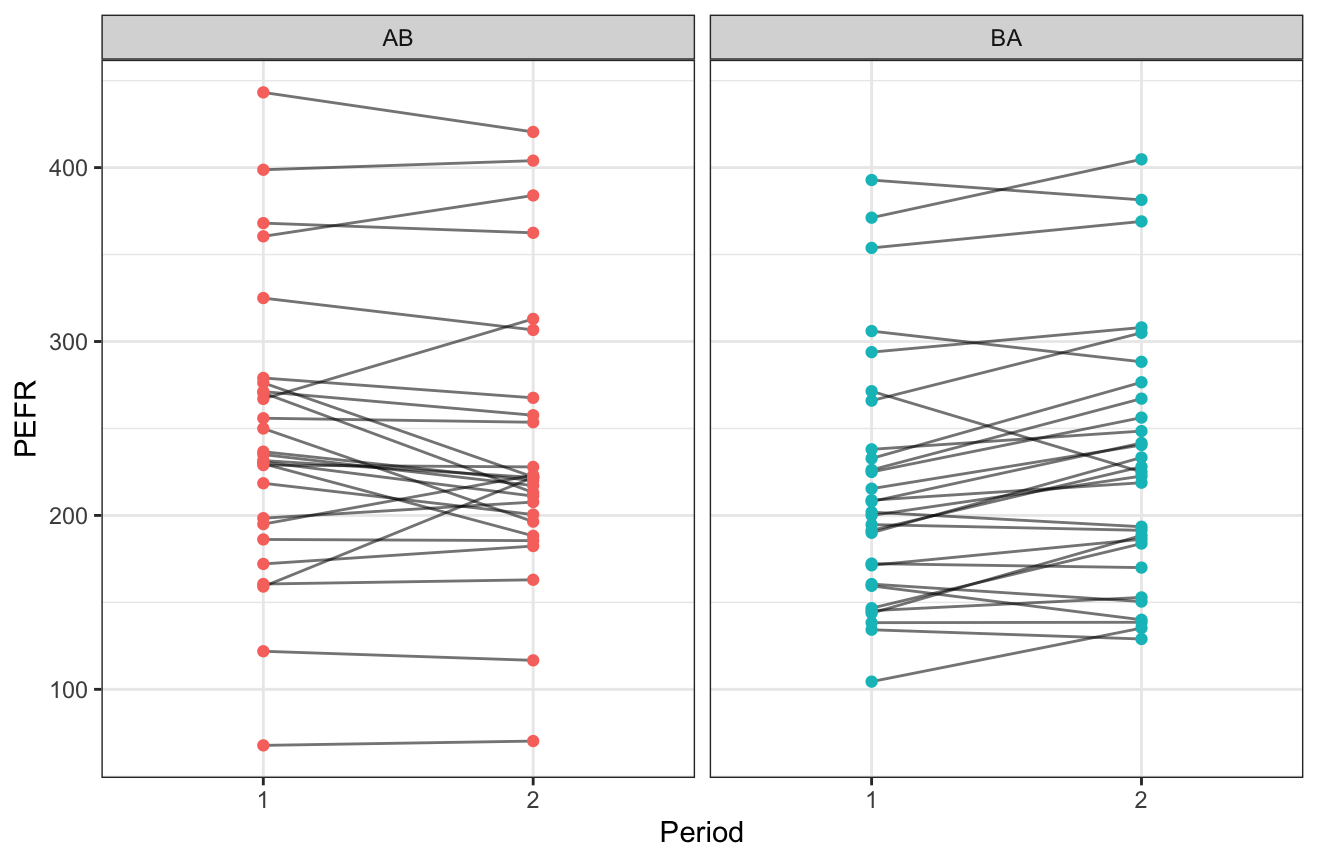
\includegraphics[width=0.85\linewidth]{report/figures/subjectProfilesPlot.png}
    \caption{Subject-Profile Plot}
    \label{fig:subjectprofile}
\end{figure}
\begin{figure}[ht]
    \centering
    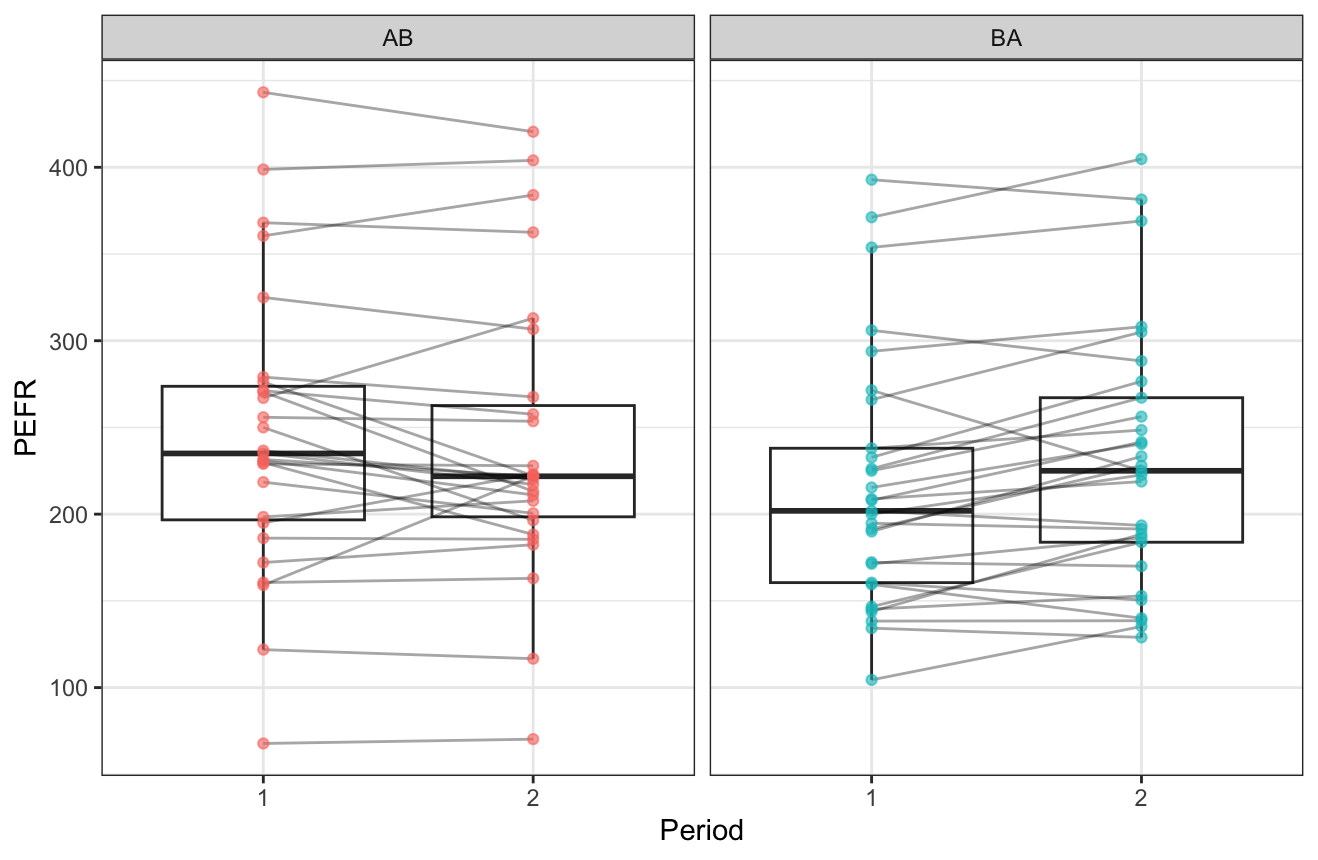
\includegraphics[width=0.85\linewidth]{report/figures/pairedboxplot.png}
    \caption{Paired Boxplot}
    \label{fig:pairedboxplot}
\end{figure}

Finally, the summary table \ref{summaryTable} can be visualised using a groups-by-periods plot, as shown in figure \ref{fig:groupsbyperiods}.
\begin{figure}[ht]
    \centering
    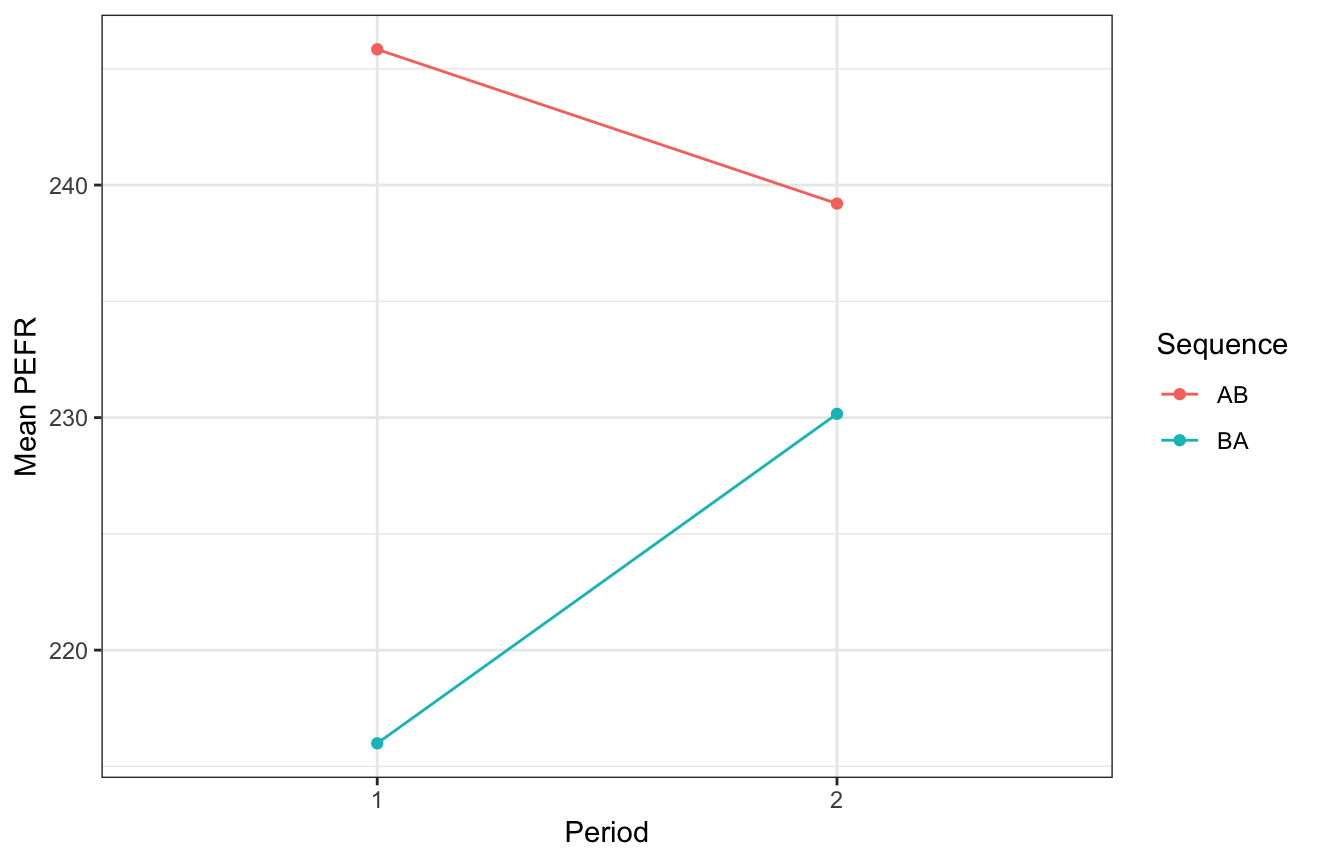
\includegraphics[width=0.85\linewidth]{report/figures/groupsByPeriodsPlot.png}
    \caption{Groups-by-Periods Plot}
    \label{fig:groupsbyperiods}
\end{figure}

\chapter{Analysis of 2x2 Cross-over Trials}

\section{Matched-Pairs \textit{t}-Test}
The most straightforward analysis for a 2x2 cross-over trial uses a matched-pairs \textit{t}-test, which takes advantage of the paired structure of the data (every observation in period 1 can be matched to the subject's corresponding observation in period 2) \cite{senn2002crossover}. Note that the alternative, a simple two-sample t-test, would give the same result as if the experiment had been carried out as a parallel group trial, as the paired structure of the cross-over design would be ignored. First we will introduce some basic notation:
\begin{itemize}
    \item $n$: number of subjects
    \item $y_{A_k}$, $y_{B_k}$: measured outcomes for subject $k$ ($k=1,\cdots,n$) after treatments $A$ and $B$ respectively.
    \item $d_k$: cross-over difference (i.e. difference between treatments) for subject $k$ ($k=1,\cdots,n$), defined as $d_k := y_{A_k}-y_{B_k}$.
\end{itemize}
And then the mean cross-over difference $\bar{d} := \frac{1}{n}\sum_{i=1}^{n}d_k$ is an estimator for the true treatment effect (or difference) $\tau$. The matched-pairs \textit{t}-test then simply involves testing the hypothesis $H_0: \tau = 0$ against $H_1: \tau \neq 0$, by computing a t-statistic and comparing it against the corresponding critical value \cite{senn2002crossover}:
\begin{align*}
    \bar{d} &:= \frac{1}{n}\sum_{i=1}^{n}d_k \\
    s &= \sqrt{\frac{1}{n-1}\sum_{i=1}^{n}(d_k-\bar{d})^2} \\
    \widehat{se(\bar{d})} &= \frac{s}{\sqrt{n}} \\
    \implies \frac{\bar{d}}{\widehat{se(\bar{d})}} &\sim t_{n-1}
\end{align*}

\subsection{Assumptions}
This method involves two important assumptions:
\begin{itemize}
    \item Cross-over differences $d_k$ are independently and randomly distributed about the true treatment effect $\tau$.
    \item Cross-over differences $d_k$ are distributed approximately normally.
\end{itemize}
The most important assumption is the first one, and there are a number of situations which could cause it to be violated:

\subsubsection{Period effect}
A period effect is present when there is a trend over time affecting the experiment as a whole. Under unbalanced allocation between treatment groups, this introduces bias to the treatment effect estimates. More generally, this can also cause us to overestimate the influence of random variation, as systematic changes between periods would be incorrectly "ascribed to random variation" \cite{senn2002crossover}.

\subsubsection{Sequence Effect}
Results may be affected by the sequence that subjects are assigned to. However, under successful randomisation, we can assume that there is no sequence effect \cite{lim2021considerations} (recalling that in a cross-over design, only the \textit{sequence} of treatments is randomised). Note that this assumption cannot be tested statistically \cite{lim2021considerations}.

\subsubsection{Period-by-treatment interaction \& carryover}
Period-by-treatment interaction occurs when the effect of the treatment varies with the period in which it is given, which could affect the cross-over difference observations. As discussed in chapter 1, presence of a carryover effect introduces significant bias to the cross-over differences.

\subsubsection{Patient-by-treatment interaction}
Patient-by-treatment interaction occurs when the effect of the treatment varies from patient to patient. This effect increases variability and causes results to be difficult to interpret, and requires a more complex trial design (administering the same treatment multiple times) to investigate further \cite{senn2002crossover}.

\subsubsection{Patient-by-period interaction}
Further complication occurs if patients are subject to period effects which are different for each patient, known as a patient-by-period interaction. Once again this adds to the variance and difficulty of interpretation.

Patient-by-period and patient-by-treatment interactions do not necessarily threaten the validity of the experiment, but they do increase variance and reduce ease of interpretation. As discussed above, period-by-treatment interactions (including carry-over) are best addressed by careful trial design, but are also the fundamental drawbacks to the cross-over design \cite{senn2002crossover}. If present, they seriously threaten the validity of subsequent analysis. Period and sequence effects, whilst not ideal, can be adjusted for using more complex models, which are demonstrated later in this chapter.

\section{Linear Models}
The issues with the matched-pairs \textit{t}-test, and the cross-over design as a whole, are better addressed within the framework of a linear model. This allows us to control for period and sequence effects, whilst also taking into account the within-subject differences. It also allows scope to include other variables of interest as covariates, such as sex and age.

The general framework for a cross-over trial model is shown in equation \ref{mixed_model}; some decisions need to be made on how to treat each individual variable to then implement a regression.

\begin{equation}
    Y_{ijk} = \mu + \tau_{jk} + \pi_j + \lambda_{j-1,k} + \gamma_k + s_{ik} + \epsilon_{ijk}
    \label{mixed_model}
\end{equation}
where $Y_{ijk}$ is the response of the $i$th subject in the $k$th sequence at the $j$th period. The model then includes the direct treatment effect $\tau_{jk}$, period effect $\pi_j$, carryover effect $\lambda_{j-1,k}$, sequence effect $\gamma_k$ and subject effects $s_{ik}$. The errors $\epsilon_{ijk}$ are i.i.d. with mean 0 and variance $\sigma^2_s$ \cite{lim2021considerations}.

The direct treatment effect, period effect and sequence effect should all be considered as fixed effects \cite{lim2021considerations}. As mentioned in the preceding discussion about carryover effect, it should be mitigated at the experiment design stage, as its presence seriously threatens the validity of the trial and post-hoc analysis. Furthermore, in the 2x2 cross-over design specifically, the carryover effect is inherent in the sequence \cite{lim2021considerations}. Hence in the regression models below, no carryover term is included, but instead we include a term for the sequence effect.

If we assume the subject effects $s_{ik}$ to be unknown fixed parameters, the regression will only use information from within-subject comparisons. Alternatively, when subject totals are judged to contain useful information, the subject effects should be treated as random effects as part of a random intercepts mixed model (see below) \cite{jones2003design}.

The regression model for the former case, treating subject effects as unknown fixed parameters, is shown in equation \ref{fixedmodelregression}, and can be estimated using the standard OLS method.

\begin{equation}
     Y = \beta_0 + \beta_1 T + \beta_2 P + \beta_3 Se + \beta_4 Su + \epsilon
     \label{fixedmodelregression}
\end{equation}
where $Y$ is the outcome variable, $T$ is the treatment administered, $P$ is the period, $Se$ is the sequence, and $Su$ is the subject. Notice that $\beta_1$ represents the direct treatment effect.

\subsection{ANOVA on Other Effects}
Before analysing the direct treatment effect, we must first verify that the aforementioned effects (other than the treatment effect) do not appear in the trial data. This can be done by applying analysis of variance (ANOVA) to model \ref{fixedmodelregression}. An example ANOVA table on 2x2 cross-over trial data from Senn and Auclair \cite{senn1990graphical} is shown in table \ref{anovaTable}.

% latex table generated in R 4.3.3 by xtable 1.8-4 package
% Mon Aug  5 15:30:30 2024
\begin{table}[ht]
\centering
\begin{tabular}{lrrrrr}
  \hline
 & Df & Sum Sq & Mean Sq & F value & Pr($>$F) \\ 
  \hline
Treat & 1 & 13388.46 & 13388.46 & 17.84 & 0.0014 \\ 
  Period & 1 & 1632.07 & 1632.07 & 2.17 & 0.1683 \\ 
  Sequence & 1 & 335.19 & 335.19 & 0.45 & 0.5177 \\ 
  Subject & 11 & 114878.27 & 10443.48 & 13.92 & 0.0001 \\ 
  Residuals & 11 & 8254.46 & 750.41 &  &  \\ 
   \hline
\end{tabular}
\caption{Example ANOVA Table for 2x2 Cross-over Trial} 
\label{anovaTable}
\end{table}



Notice that in this example, neither the sequence (i.e. carryover) or period effects are statistically significant, indicating we can reliably estimate the treatment effect \cite{lim2021considerations}.

\subsection{Mixed Model for Cross-over Design}
When between-subject differences are judged to be relevant, a mixed model (more specifically a random intercepts model) is superior to the simple linear regression model \ref{fixedmodelregression} for 2x2 cross-over trials \cite{jones2003design}. In a random intercepts mixed model, treating subject effects as random effects, we include a term for the unique effect of each subject, so that we have subject-specific intercepts \cite{mixedmodelsR}. The corresponding regression is demonstrated in equation \ref{mixedmodelregression}, and can be estimated using the Restricted Maximum Likelihood (REML) method \cite{jones2003design}.

\begin{equation}
   Y = \beta_0 + \beta_1 T + \beta_2 P + \beta_3 Se + \beta_{subject} + \epsilon
   \label{mixedmodelregression}
\end{equation}

Additional subject-level covariates, such as sex and age, can be added as covariates in the same way as for a simple linear regression.

\subsection{Adjusting for Baseline Values}
In pre-post designs, analysis of covariance (ANCOVA), whereby the pre-test (baseline) measurement is included as a covariate, is the most efficient method of analysis \cite{wan2021statistical}. For 2x2 cross-over trials, we can further improve model efficiency by taking baseline measurements into account (when available). This requires that baseline measurements be taken for each subject prior to each treatment period, so that a total of 4 measurements per subject are taken over the course of the trial.

Mehrotra \cite{mehrotra2014} concludes that the most efficient method to interpret baseline measurements is to include within-subject difference in baselines as a covariate, interacting with period. This is shown as part of the simple linear regression in equation \ref{baselinemodel}, and as part of the mixed model in equation \ref{baselinemixedmodel}.

\begin{equation}
    Y = \beta_0 + \beta_1 T + \beta_2 P \cdot X_{diff} + \beta_3 P +
    \beta_4 X_{diff} + \beta_5 Se + \beta_6 Su + \epsilon
    \label{baselinemodel}
\end{equation}

\begin{equation}
    Y = \beta_0 + \beta_1 T + \beta_2 P \cdot X_{diff} + \beta_3 P +
    \beta_4 X_{diff} + \beta_5 Se + \beta_{subject} + \epsilon
    \label{baselinemixedmodel}
\end{equation}
Where $X_{diff} := X_1 - X_2$, with $X_1$ and $X_2$ being the baseline measurements before treatment periods 1 and 2 respectively.

\subsection{Verifying Assumptions}
Before analysing model results, it is important to verify that some key assumptions hold, to ensure validity of the fitted model. The following assumptions must hold for either the simple regression or the mixed model to be valid for a 2x2 cross-over trial:
\begin{itemize}
    \item Linearity
    \item Homoscedasticity
    \item Normality of residuals
\end{itemize}
Linearity is not a concern as the independent variable (treatment) only takes 2 values. Homoscedasticity and normality of residuals are best verified graphically using a scatter plot of residuals against fitted values and a Q-Q plot, respectively.
\begin{figure}[ht]
    \centering
    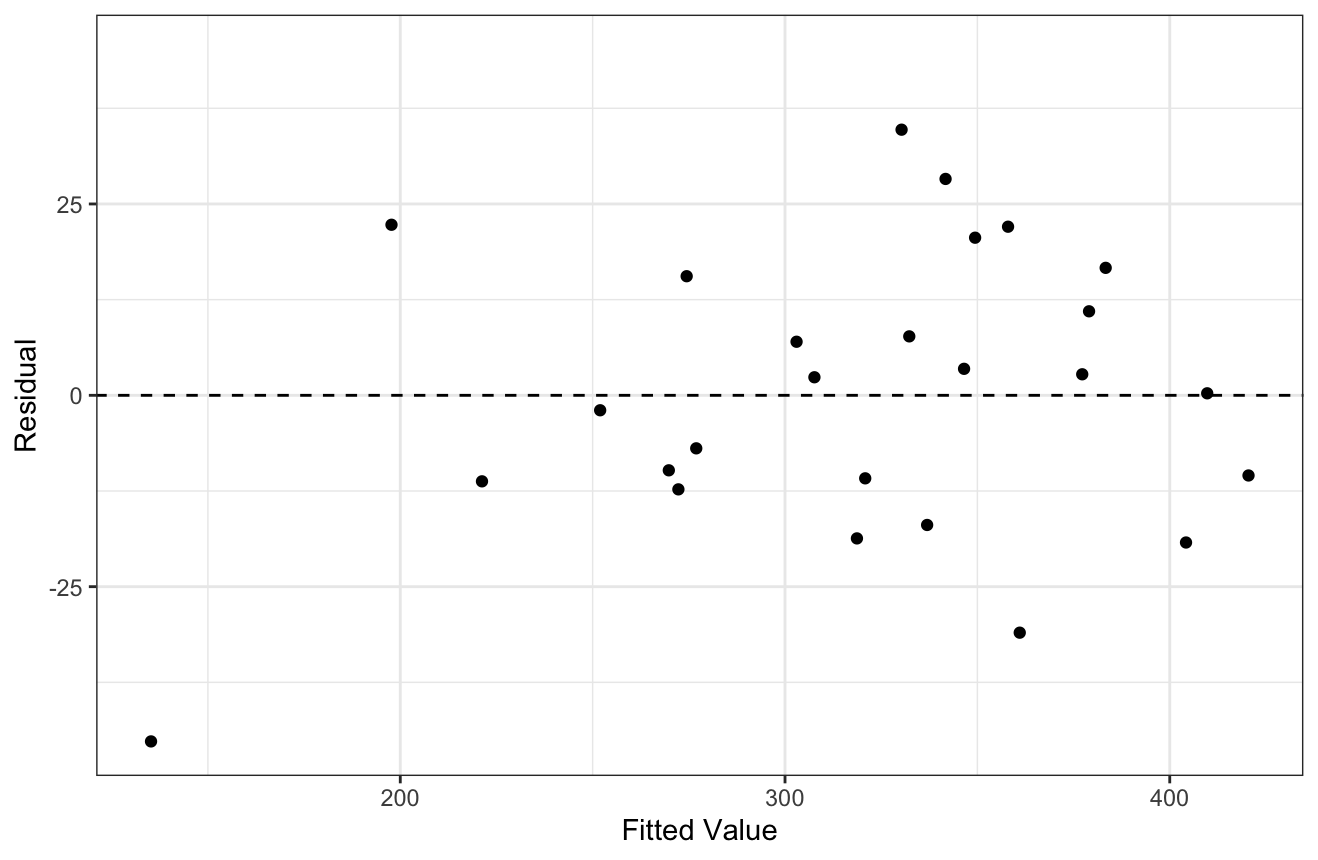
\includegraphics[width=0.85\linewidth]{report/figures/homoscedasticityPlot.png}
    \caption{Plot to verify homoscedasticity}
    \label{fig:homoscedasticity}
\end{figure}
\begin{figure}[ht]
    \centering
    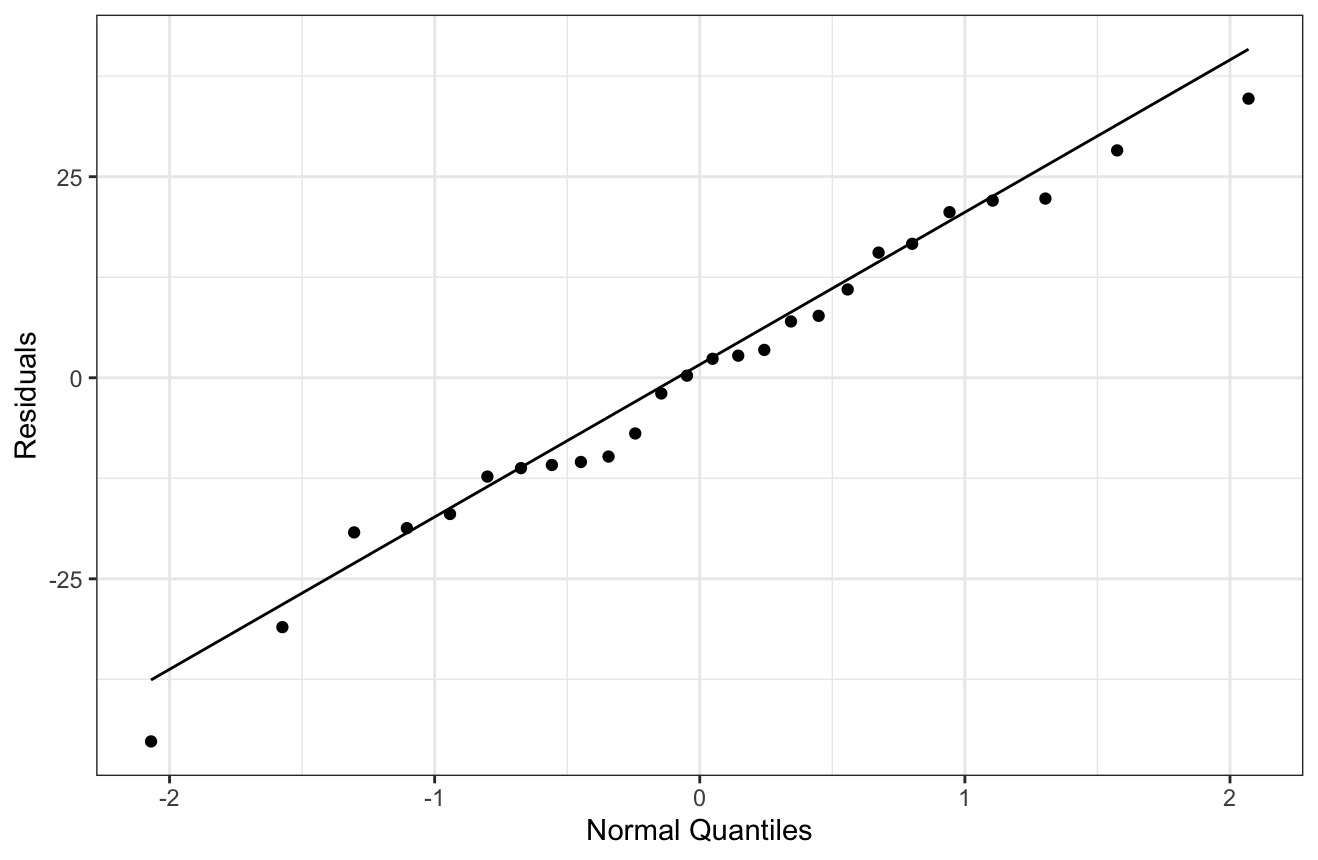
\includegraphics[width=0.85\linewidth]{report/figures/qqplot.png}
    \caption{Q-Q Plot to verify normality of residuals}
    \label{fig:qqplot}
\end{figure}

\subsection{Analysing Results}
Whichever model is chosen, the estimated coefficients and their corresponding p-values should be reported, as in table \ref{modelTable}. We can then use the p-values to determine the existence of a treatment effect (or difference between treatments). It is also useful to report the least squares (LS) means (see table \ref{lsMeansTable}) for each treatment, which provide an insightful summary of the differences between treatments, and hence the magnitude of the treatment effect (if any).

% latex table generated in R 4.3.3 by xtable 1.8-4 package
% Mon Aug  5 19:20:34 2024
\begin{table}[ht]
\centering
\begin{tabular}{rlllrrrrr}
  \hline
 & effect & group & term & estimate & std.error & statistic & df & p.value \\ 
  \hline
1 & fixed &  & (Intercept) & 337.14 & 28.28 & 11.92 & 12.57 & 0.00 \\ 
  2 & fixed &  & TreatSal & -46.61 & 10.78 & -4.32 & 11.00 & 0.00 \\ 
  3 & fixed &  & Period2 & 15.89 & 10.78 & 1.47 & 11.00 & 0.17 \\ 
  4 & fixed &  & SequenceSal-For & -7.20 & 40.20 & -0.18 & 11.00 & 0.86 \\ 
  5 & ran\_pars & Subject & sd\_\_(Intercept) & 69.62 &  &  &  &  \\ 
  6 & ran\_pars & Residual & sd\_\_Observation & 27.39 &  &  &  &  \\ 
   \hline
\end{tabular}
\caption{Example Estimates for 2x2 Cross-over Trial} 
\label{modelTable}
\end{table}


% latex table generated in R 4.3.3 by xtable 1.8-4 package
% Mon Aug  5 21:18:14 2024
\begin{table}[ht]
\centering
\begin{tabular}{l|rrrrr}
  \hline
Treat & emmean & SE & df & lower.CL & upper.CL \\ 
  \hline
For & 341.49 & 20.81 & 12.57 & 296.37 & 386.60 \\ 
  Sal & 294.88 & 20.81 & 12.57 & 249.77 & 340.00 \\ 
   \hline
\end{tabular}
\caption{Example LS Means for 2x2 Cross-over Trial} 
\label{lsMeansTable}
\end{table}

\chapter{Worked Example} \label{example}

	% Begin Bibliography
	{
	
	\bibliography{references}
	\bibliographystyle{ieeetr}
	
	}
	
\end{document}
